% !TEX TS-program = pdflatex
\documentclass[11pt]{article}

% -------------------- Packages --------------------
\usepackage[a4paper,margin=1in]{geometry}
\usepackage{amsmath,amssymb}
\usepackage[T1]{fontenc}
\usepackage{lmodern}
\usepackage{xcolor}
\usepackage{tcolorbox}
\tcbuselibrary{skins,breakable}
\usepackage{enumitem}
\usepackage{hyperref}
\usepackage{tikz}
\usetikzlibrary{calc,patterns}

\pagestyle{empty}

% -------------------- Dark Theme Colors --------------------
\definecolor{bg}{HTML}{000000}
\definecolor{pairbg}{HTML}{121212}
\definecolor{solbg}{HTML}{0A0A0A}
\definecolor{border}{HTML}{2A2A2A}
\definecolor{text}{HTML}{FFFFFF}
\definecolor{muted}{HTML}{C9CDD3}
\definecolor{gold}{HTML}{FFD700}
\definecolor{green}{HTML}{4ADE80}
\definecolor{cyan}{HTML}{38BDF8}

\pagecolor{bg}
\color{text}

\hypersetup{
  colorlinks=true,
  linkcolor=cyan,
  urlcolor=cyan
}

\setlength{\parindent}{0pt}
\setlength{\parskip}{10pt}

\setlist[itemize]{left=1.4em,itemsep=6pt,topsep=6pt}
\setlist[enumerate]{left=1.6em,itemsep=4pt,topsep=4pt}

% -------------------- tcolorbox Base --------------------
\tcbset{
  enhanced,
  breakable,
  arc=12pt,
  boxrule=0.8pt,
  left=16pt,right=16pt,top=12pt,bottom=12pt
}

\newtcolorbox{QAPair}[1]{%
  colback=pairbg,
  colbacklower=solbg,
  colframe=border,
  coltext=text,
  title=\textcolor{gold}{\bfseries #1},
  fonttitle=\bfseries,
  coltitle=text,
  segmentation style={draw=border, dashed, line width=0.6pt},
}

\newtcolorbox{QuickBox}{%
  colback=pairbg,
  colframe=cyan,
  coltext=text,
  fontupper=\color{text},
  borderline north={4pt}{0pt}{cyan},
  arc=14pt,
  boxrule=0.8pt
}

% Helper for step headings
\newcommand{\Step}[1]{\textcolor{muted}{\textbf{Step #1:}}}

% -------------------- TikZ Styles --------------------
\tikzset{
  vennCircle/.style={draw=muted, line width=0.9pt},
  vennFill/.style={fill=cyan, fill opacity=0.22},
  vennLabel/.style={text=text, font=\small},
  vennText/.style={text=text, font=\small}
}

% ============================================================
\begin{document}

\begin{center}
{\LARGE\bfseries \textcolor{gold}{Miscellaneous Exercise 3 --- Solutions}}\\[-2pt]
\end{center}

\begin{QuickBox}
{\color{cyan}\bfseries Quick formulas (useful)}\par\medskip
\begin{itemize}
\item \textbf{Set difference:} $A-B=\{x\mid x\in A \ \wedge\ x\notin B\}$.
\item \textbf{Complement:} $A\cap A^c=\varnothing$ and $A\cup A^c=U$.
\item \textbf{Cartesian product size:} If $|A|=m$, $|B|=n$ then $|A\times B|=mn$.
\item \textbf{Binary relations count:} Number of relations from $A$ to $B$ is $2^{|A\times B|}$.
\item \textbf{Inclusion--Exclusion:} $n(A\cup B)=n(A)+n(B)-n(A\cap B)$.
\end{itemize}
\end{QuickBox}

% ============================================================
% Q1 (MCQs) — Separate box for each part + step-wise explanation

\begin{QAPair}{Question 1 (i) --- MCQ}
\textcolor{gold}{\bfseries Question:} Set-builder form of $A-B$ is:\par
\begin{itemize}
\item[(a)] $\{x\mid x\in A\}$
\item[(b)] $\{x\mid x\in A \wedge x\notin B\}$
\item[(c)] $\{x\mid x\in A \wedge x\in B\}$
\item[(d)] $\{x\mid x\in B\}$
\end{itemize}
\tcblower
\textcolor{green}{\bfseries Answer:} \textbf{(b)}\par
\[
\begin{aligned}
\Step{1}\;& A-B \text{ means ``elements in }A\text{ but not in }B\text{.''}\\
\Step{2}\;& \text{So }A-B=\{x\mid x\in A \ \wedge\ x\notin B\}.\\
\Step{3}\;& \Rightarrow \text{ option (b).}
\end{aligned}
\]
\end{QAPair}

\begin{QAPair}{Question 1 (ii) --- MCQ}
\textcolor{gold}{\bfseries Question:} If $A\cup B=A$ and $A\cap B=B$, then:\par
\begin{itemize}
\item[(a)] $A\subseteq B$
\item[(b)] $A\nsubseteq B$
\item[(c)] $A\supseteq B$
\item[(d)] $A\neq B$
\end{itemize}
\tcblower
\textcolor{green}{\bfseries Answer:} \textbf{(c)}\par
\[
\begin{aligned}
\Step{1}\;& A\cap B=B \ \Rightarrow\ \text{every element of }B\text{ is in }A.\\
\Step{2}\;& \Rightarrow\ B\subseteq A \ \Leftrightarrow\ A\supseteq B.\\
\Step{3}\;& \Rightarrow \text{ option (c).}
\end{aligned}
\]
\end{QAPair}

\begin{QAPair}{Question 1 (iii) --- MCQ}
\textcolor{gold}{\bfseries Question:} If $A\subset B$ then $A-B=$\par
\begin{itemize}
\item[(a)] $A$
\item[(b)] $B$
\item[(c)] $\varnothing$
\item[(d)] $B-A$
\end{itemize}
\tcblower
\textcolor{green}{\bfseries Answer:} \textbf{(c)}\par
\[
\begin{aligned}
\Step{1}\;& A\subset B \Rightarrow \text{every element of }A\text{ is already in }B.\\
\Step{2}\;& A-B=\{x\in A: x\notin B\}. \\
\Step{3}\;& \text{But there is no such }x,\ \Rightarrow\ A-B=\varnothing.\\
\Step{4}\;& \Rightarrow \text{ option (c).}
\end{aligned}
\]
\end{QAPair}

\begin{QAPair}{Question 1 (iv) --- MCQ}
\textcolor{gold}{\bfseries Question:} If $A-B=B-A=\varnothing$, then:\par
\begin{itemize}
\item[(a)] $A=B$
\item[(b)] $B\subseteq A$
\item[(c)] $A\subseteq B$
\item[(d)] all a, b \& c
\end{itemize}
\tcblower
\textcolor{green}{\bfseries Answer:} \textbf{(d)}\par
\[
\begin{aligned}
\Step{1}\;& A-B=\varnothing \Rightarrow A\subseteq B.\\
\Step{2}\;& B-A=\varnothing \Rightarrow B\subseteq A.\\
\Step{3}\;& A\subseteq B \ \text{and}\ B\subseteq A \Rightarrow A=B.\\
\Step{4}\;& \text{So (a), (b), (c) are all true} \Rightarrow \text{(d).}
\end{aligned}
\]
\end{QAPair}

\begin{QAPair}{Question 1 (v) --- MCQ}
\textcolor{gold}{\bfseries Question:} Set of common elements of $A$ and $A^c$ is \_\_\_\_ set.\par
\begin{itemize}
\item[(a)] infinite
\item[(b)] null
\item[(c)] universal
\item[(d)] singleton
\end{itemize}
\tcblower
\textcolor{green}{\bfseries Answer:} \textbf{(b)}\par
\[
\begin{aligned}
\Step{1}\;& A^c \text{ means elements \emph{not} in }A.\\
\Step{2}\;& A\cap A^c=\varnothing \quad (\text{nothing can be in }A\text{ and not in }A).\\
\Step{3}\;& \Rightarrow \text{null set }(\varnothing)\Rightarrow \text{ option (b).}
\end{aligned}
\]
\end{QAPair}

\begin{QAPair}{Question 1 (vi) --- MCQ}
\textcolor{gold}{\bfseries Question:} Set of real numbers can be written in:\par
\begin{itemize}
\item[(a)] tabular form
\item[(b)] descriptive form
\item[(c)] set-builder form
\item[(d)] both b and c
\end{itemize}
\tcblower
\textcolor{green}{\bfseries Answer:} \textbf{(d)}\par
\[
\begin{aligned}
\Step{1}\;& \mathbb{R} \text{ is infinite, so we cannot list it completely (not tabular).}\\
\Step{2}\;& \text{We can describe it in words (descriptive form).}\\
\Step{3}\;& \text{We can also write it using a rule (set-builder form).}\\
\Step{4}\;& \Rightarrow \text{both (b) and (c) are correct} \Rightarrow \text{(d).}
\end{aligned}
\]
\end{QAPair}

\begin{QAPair}{Question 1 (vii) --- MCQ}
\textcolor{gold}{\bfseries Question:} If $R=\{(2,1),(4,3),(2,2)\}$, then $\mathrm{Dom}\,R=$\par
\begin{itemize}
\item[(a)] $\{2,4,2\}$
\item[(b)] $\{2,4\}$
\item[(c)] $\{1,3,2\}$
\item[(d)] none of these
\end{itemize}
\tcblower
\textcolor{green}{\bfseries Answer:} \textbf{(b)}\par
\[
\begin{aligned}
\Step{1}\;& \mathrm{Dom}(R)=\{\text{first components of ordered pairs}\}.\\
\Step{2}\;& \text{First components are }2,4,2.\\
\Step{3}\;& \text{As a set (no repeats): }\{2,4\}.\\
\Step{4}\;& \Rightarrow \text{ option (b).}
\end{aligned}
\]
\end{QAPair}

\begin{QAPair}{Question 1 (viii) --- MCQ}
\textcolor{gold}{\bfseries Question:} If $R=\{(a,b)\mid a,b\in\mathbb{Z}\ \wedge\ a+b=0\}$, then:\par
\begin{itemize}
\item[(a)] $\mathrm{Dom}\,R \subset \mathrm{Range}\,R$
\item[(b)] $\mathrm{Range}\,R \subset \mathrm{Dom}\,R$
\item[(c)] $\mathrm{Dom}\,R = \mathrm{Range}\,R$
\item[(d)] none of these
\end{itemize}
\tcblower
\textcolor{green}{\bfseries Answer:} \textbf{(c)}\par
\[
\begin{aligned}
\Step{1}\;& a+b=0 \Rightarrow b=-a.\\
\Step{2}\;& \text{For every }a\in\mathbb{Z},\ b=-a\in\mathbb{Z}\text{ exists } \Rightarrow a \text{ is in the domain.}\\
\Step{3}\;& \text{So }\mathrm{Dom}(R)=\mathbb{Z}.\\
\Step{4}\;& \text{Similarly, for any }b\in\mathbb{Z},\ a=-b\in\mathbb{Z}\text{ exists } \Rightarrow \mathrm{Range}(R)=\mathbb{Z}.\\
\Step{5}\;& \Rightarrow \mathrm{Dom}(R)=\mathrm{Range}(R) \Rightarrow \text{(c).}
\end{aligned}
\]
\end{QAPair}

\begin{QAPair}{Question 1 (ix) --- MCQ}
\textcolor{gold}{\bfseries Question:} If $R=\{(a,b)\mid a,b\in\mathbb{N}\ \wedge\ a\times b=12\}$, then tabular form of $R$ is:\par
\begin{itemize}
\item[(a)] $\{(1,12),(2,6),(3,4),(4,3),(6,2),(12,1)\}$
\item[(b)] $\{(1,12),(2,6),(3,4)\}$
\item[(c)] $\{(12,1),(6,2),(4,3)\}$
\item[(d)] $\{(1,12),(4,3),(2,6)\}$
\end{itemize}
\tcblower
\textcolor{green}{\bfseries Answer:} \textbf{(a)}\par
\[
\begin{aligned}
\Step{1}\;& ab=12 \text{ with }a,b\in\mathbb{N} \Rightarrow \text{list all factor pairs of }12.\\
\Step{2}\;& 12=1\cdot12=2\cdot6=3\cdot4.\\
\Step{3}\;& \text{Include both orders for ordered pairs:}\\
& (1,12),(12,1),(2,6),(6,2),(3,4),(4,3).\\
\Step{4}\;& \Rightarrow \text{ option (a).}
\end{aligned}
\]
\end{QAPair}

\begin{QAPair}{Question 1 (x) --- MCQ}
\textcolor{gold}{\bfseries Question:} If $n(A)=p$, then $n(A\times A)=$\par
\begin{itemize}
\item[(a)] $p$
\item[(b)] $2p$
\item[(c)] $2p^2$
\item[(d)] $p^2$
\end{itemize}
\tcblower
\textcolor{green}{\bfseries Answer:} \textbf{(d)}\par
\[
\begin{aligned}
\Step{1}\;& |A\times A|=|A|\cdot|A|.\\
\Step{2}\;& =p\cdot p=p^2.\\
\Step{3}\;& \Rightarrow \text{ option (d).}
\end{aligned}
\]
\end{QAPair}

\begin{QAPair}{Question 1 (xi) --- MCQ}
\textcolor{gold}{\bfseries Question:} If $n(B)=t$, then number of binary relations in $B\times B$ is:\par
\begin{itemize}
\item[(a)] $t$
\item[(b)] $t^2$
\item[(c)] $2^t$
\item[(d)] $2^{t^2}$
\end{itemize}
\tcblower
\textcolor{green}{\bfseries Answer:} \textbf{(d)}\par
\[
\begin{aligned}
\Step{1}\;& |B\times B|=|B|\cdot|B|=t^2.\\
\Step{2}\;& \text{A relation is any subset of }B\times B.\\
\Step{3}\;& \text{Number of subsets of a set with }t^2\text{ elements is }2^{t^2}.\\
\Step{4}\;& \Rightarrow \text{ option (d).}
\end{aligned}
\]
\end{QAPair}

% ============================================================
% Q2
\begin{QAPair}{Question 2 (i)--(v)}
\textcolor{gold}{\bfseries Question:} If $R=\{a,f,h,s\}$ and $S=\{b,e,j,n\}$, then answer (i)--(v).\\
\tcblower
\textcolor{green}{\bfseries Answer:}

\[
|R|=4,\quad |S|=4 \;\Rightarrow\; |R\times S|=4\cdot 4=16.
\]

\begin{enumerate}[label=\textbf{(\roman*)}]
\item \textbf{Number of binary relations in $R\times S$:}
\[
\#\text{relations} = 2^{|R\times S|}=2^{16}.
\]

\item \textbf{Any 3 binary relations from $R\times S$ (examples):}
\[
\begin{aligned}
\mathcal{R}_1&=\{(a,b)\},\\
\mathcal{R}_2&=\{(f,e),(h,j)\},\\
\mathcal{R}_3&=\{(s,n),(a,e),(h,b)\}.
\end{aligned}
\]

\item \textbf{A relation whose domain is exactly $R$:}
\[
\mathcal{R}_D=\{(a,b),(f,b),(h,b),(s,b)\}.
\]
Then $\mathrm{Dom}(\mathcal{R}_D)=R$.

\item \textbf{A relation whose range is exactly $S$:}
\[
\mathcal{R}_R=\{(a,b),(a,e),(a,j),(a,n)\}.
\]
Then $\mathrm{Range}(\mathcal{R}_R)=S$.

\item \textbf{A relation whose domain is $R$ and range is $S$:}
\[
\mathcal{R}=\{(a,b),(f,e),(h,j),(s,n)\}.
\]
\end{enumerate}
\end{QAPair}

% ============================================================
% Q3
\begin{QAPair}{Question 3 (Shading on the given Venn diagram)}
\textcolor{gold}{\bfseries Question:} Shade $A\cup(B\cap C)$, $A\cap(B\cup C)$, $A-(B\cap C)$ and $B-(A\cup C)$.\\
\tcblower
\textcolor{green}{\bfseries Answer:}

From the diagram:
\[
A=\{a,b,c,d\},\quad B=\{e,f,h\},\quad C=\{a,c,e,i,j\}.
\]
So $B\cap C=\{e\}$ and $A\cap C=\{a,c\}$.

\begin{enumerate}[label=\textbf{(\roman*)}]
\item $A\cup(B\cap C)=A\cup\{e\}=\{a,b,c,d,e\}$.
\item $A\cap(B\cup C)=A\cap C=\{a,c\}$.
\item $A-(B\cap C)=A-\{e\}=A=\{a,b,c,d\}$.
\item $B-(A\cup C)=\{e,f,h\}-\{a,b,c,d,e,i,j\}=\{f,h\}$.
\end{enumerate}

\textcolor{muted}{(Venn diagrams showing the shaded regions)}\par\medskip

% ---- (i) A ∪ (B ∩ C)
\textcolor{gold}{\bfseries (i) $A\cup(B\cap C)$}\par
\begin{center}
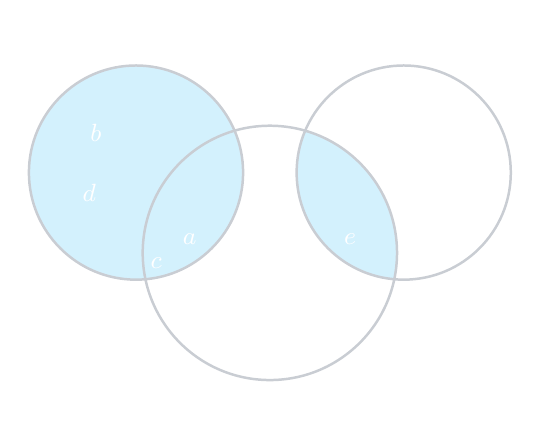
\begin{tikzpicture}[scale=0.85]
  \def\rA{1.6}
  \def\rB{1.6}
  \def\rC{1.9}
  \coordinate (A) at (-2,0);
  \coordinate (B) at (2,0);
  \coordinate (C) at (0,-1.2);

  \fill[vennFill] (A) circle (\rA);

  \begin{scope}
    \clip (B) circle (\rB);
    \fill[vennFill] (C) circle (\rC);
  \end{scope}

  \draw[vennCircle] (A) circle (\rA);
  \draw[vennCircle] (B) circle (\rB);
  \draw[vennCircle] (C) circle (\rC);

  \node[vennLabel] at (-2,1.9) {$A$};
  \node[vennLabel] at (2,1.9) {$B$};
  \node[vennLabel] at (0,-3.3) {$C$};

  \node[vennText] at (-2.6,0.6) {$b$};
  \node[vennText] at (-2.7,-0.3) {$d$};
  \node[vennText] at (-1.2,-1.0) {$a$};
  \node[vennText] at (-1.7,-1.35) {$c$};

  \node[vennText] at (1.2,-1.0) {$e$};
  \node[vennText] at (2.6,0.6) {$f$};
  \node[vennText] at (2.7,-0.3) {$h$};

  \node[vennText] at (-0.5,-2.25) {$i$};
  \node[vennText] at (0.5,-2.25) {$j$};
\end{tikzpicture}
\end{center}

% ---- (ii) A ∩ (B ∪ C) = A ∩ C
\textcolor{gold}{\bfseries (ii) $A\cap(B\cup C)$}\par
\begin{center}
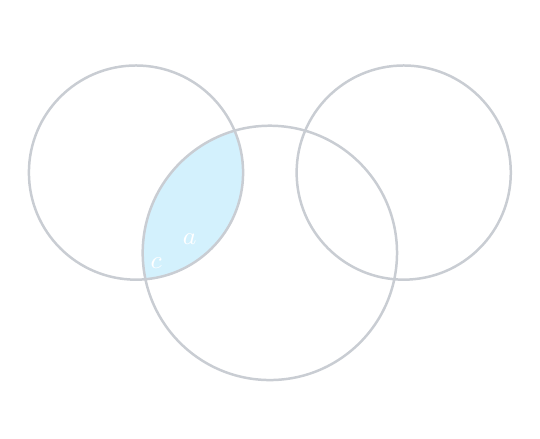
\begin{tikzpicture}[scale=0.85]
  \def\rA{1.6}
  \def\rB{1.6}
  \def\rC{1.9}
  \coordinate (A) at (-2,0);
  \coordinate (B) at (2,0);
  \coordinate (C) at (0,-1.2);

  \begin{scope}
    \clip (A) circle (\rA);
    \fill[vennFill] (C) circle (\rC);
  \end{scope}

  \draw[vennCircle] (A) circle (\rA);
  \draw[vennCircle] (B) circle (\rB);
  \draw[vennCircle] (C) circle (\rC);

  \node[vennLabel] at (-2,1.9) {$A$};
  \node[vennLabel] at (2,1.9) {$B$};
  \node[vennLabel] at (0,-3.3) {$C$};

  \node[vennText] at (-2.6,0.6) {$b$};
  \node[vennText] at (-2.7,-0.3) {$d$};
  \node[vennText] at (-1.2,-1.0) {$a$};
  \node[vennText] at (-1.7,-1.35) {$c$};

  \node[vennText] at (1.2,-1.0) {$e$};
  \node[vennText] at (2.6,0.6) {$f$};
  \node[vennText] at (2.7,-0.3) {$h$};

  \node[vennText] at (-0.5,-2.25) {$i$};
  \node[vennText] at (0.5,-2.25) {$j$};
\end{tikzpicture}
\end{center}

% ---- (iii) A - (B ∩ C) = A
\textcolor{gold}{\bfseries (iii) $A-(B\cap C)$}\par
\begin{center}
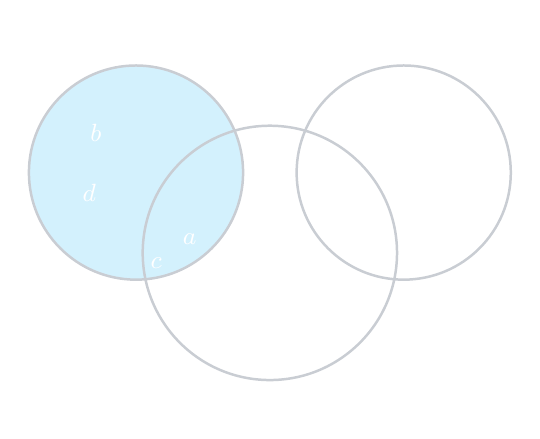
\begin{tikzpicture}[scale=0.85]
  \def\rA{1.6}
  \def\rB{1.6}
  \def\rC{1.9}
  \coordinate (A) at (-2,0);
  \coordinate (B) at (2,0);
  \coordinate (C) at (0,-1.2);

  \fill[vennFill] (A) circle (\rA);

  \draw[vennCircle] (A) circle (\rA);
  \draw[vennCircle] (B) circle (\rB);
  \draw[vennCircle] (C) circle (\rC);

  \node[vennLabel] at (-2,1.9) {$A$};
  \node[vennLabel] at (2,1.9) {$B$};
  \node[vennLabel] at (0,-3.3) {$C$};

  \node[vennText] at (-2.6,0.6) {$b$};
  \node[vennText] at (-2.7,-0.3) {$d$};
  \node[vennText] at (-1.2,-1.0) {$a$};
  \node[vennText] at (-1.7,-1.35) {$c$};

  \node[vennText] at (1.2,-1.0) {$e$};
  \node[vennText] at (2.6,0.6) {$f$};
  \node[vennText] at (2.7,-0.3) {$h$};

  \node[vennText] at (-0.5,-2.25) {$i$};
  \node[vennText] at (0.5,-2.25) {$j$};
\end{tikzpicture}
\end{center}

% ---- (iv) B - (A ∪ C) = B only (outside C)
\textcolor{gold}{\bfseries (iv) $B-(A\cup C)$}\par
\begin{center}
\begin{tikzpicture}[scale=0.85]
  \def\rA{1.6}
  \def\rB{1.6}
  \def\rC{1.9}
  \coordinate (A) at (-2,0);
  \coordinate (B) at (2,0);
  \coordinate (C) at (0,-1.2);

  \begin{scope}
    \clip (B) circle (\rB);
    \clip[even odd rule] (C) circle (\rC) (-5,-5) rectangle (5,5);
    \fill[vennFill] (B) circle (\rB);
  \end{scope}

  \draw[vennCircle] (A) circle (\rA);
  \draw[vennCircle] (B) circle (\rB);
  \draw[vennCircle] (C) circle (\rC);

  \node[vennLabel] at (-2,1.9) {$A$};
  \node[vennLabel] at (2,1.9) {$B$};
  \node[vennLabel] at (0,-3.3) {$C$};

  \node[vennText] at (-2.6,0.6) {$b$};
  \node[vennText] at (-2.7,-0.3) {$d$};
  \node[vennText] at (-1.2,-1.0) {$a$};
  \node[vennText] at (-1.7,-1.35) {$c$};

  \node[vennText] at (1.2,-1.0) {$e$};
  \node[vennText] at (2.6,0.6) {$f$};
  \node[vennText] at (2.7,-0.3) {$h$};

  \node[vennText] at (-0.5,-2.25) {$i$};
  \node[vennText] at (0.5,-2.25) {$j$};
\end{tikzpicture}
\end{center}

\end{QAPair}

% ============================================================
% Q4
\begin{QAPair}{Question 4 (Associative laws of $\cup$ and $\cap$)}
\textcolor{gold}{\bfseries Question:} Verify associative properties of union and intersection through Venn diagram for\\
$X=\{2x\mid x\in\mathbb{N}\wedge x<20\}$,\;
$Y=$ first 6 natural multiples of 3,\;
$Z=\{6x\mid x\in\mathbb{W}\wedge x<20\}$.\\
\tcblower
\textcolor{green}{\bfseries Answer:}

\[
\begin{aligned}
X&=\{2,4,6,\dots,38\},\\
Y&=\{3,6,9,12,15,18\},\\
Z&=\{0,6,12,18,24,30,36,42,\dots,114\}.
\end{aligned}
\]

\textcolor{muted}{\textbf{(a) Union (associative):}}\\
\[
(X\cup Y)\cup Z = X\cup(Y\cup Z)=X\cup Y\cup Z.
\]

\begin{center}
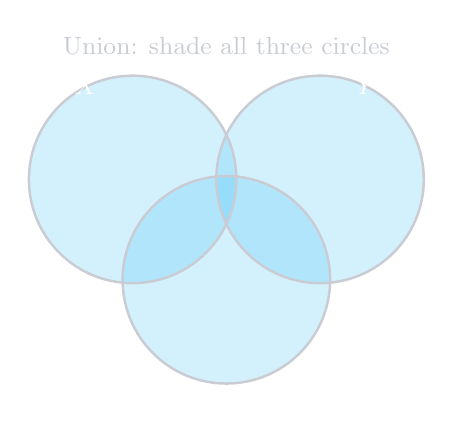
\begin{tikzpicture}[scale=0.85]
  \def\r{1.55}
  \coordinate (X) at (-1.4,0.3);
  \coordinate (Y) at (1.4,0.3);
  \coordinate (Z) at (0,-1.2);

  \fill[vennFill] (X) circle (\r);
  \fill[vennFill] (Y) circle (\r);
  \fill[vennFill] (Z) circle (\r);

  \draw[vennCircle] (X) circle (\r);
  \draw[vennCircle] (Y) circle (\r);
  \draw[vennCircle] (Z) circle (\r);

  \node[vennLabel] at (-2.1,1.7) {$X$};
  \node[vennLabel] at (2.1,1.7) {$Y$};
  \node[vennLabel] at (0,-2.9) {$Z$};
  \node[vennText, text=muted] at (0,2.3) {Union: shade all three circles};
\end{tikzpicture}
\end{center}

\textcolor{muted}{\textbf{(b) Intersection (associative):}}\\
\[
(X\cap Y)\cap Z = X\cap(Y\cap Z)=X\cap Y\cap Z.
\]
\[
X\cap Y=\{6,12,18\},\quad (X\cap Y)\cap Z=\{6,12,18\}.
\]

\begin{center}
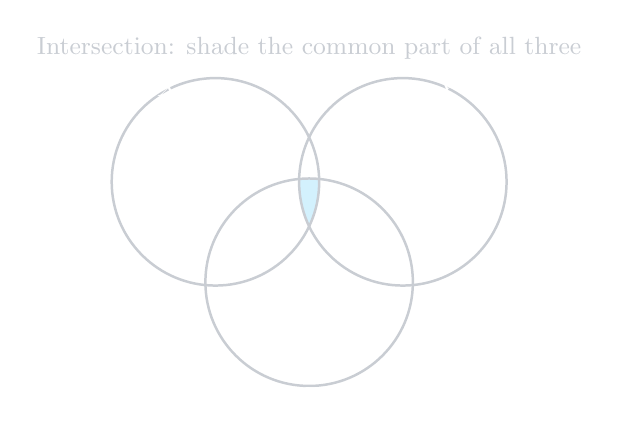
\begin{tikzpicture}[scale=0.85]
  \def\r{1.55}
  \coordinate (X) at (-1.4,0.3);
  \coordinate (Y) at (1.4,0.3);
  \coordinate (Z) at (0,-1.2);

  \begin{scope}
    \clip (X) circle (\r);
    \clip (Y) circle (\r);
    \fill[vennFill] (Z) circle (\r);
  \end{scope}

  \draw[vennCircle] (X) circle (\r);
  \draw[vennCircle] (Y) circle (\r);
  \draw[vennCircle] (Z) circle (\r);

  \node[vennLabel] at (-2.1,1.7) {$X$};
  \node[vennLabel] at (2.1,1.7) {$Y$};
  \node[vennLabel] at (0,-2.9) {$Z$};
  \node[vennText, text=muted] at (0,2.3) {Intersection: shade the common part of all three};
\end{tikzpicture}
\end{center}
\end{QAPair}

% ============================================================
% Q5
\begin{QAPair}{Question 5 (Distributive law of $\cup$ over $\cap$)}
\textcolor{gold}{\bfseries Question:} Verify distributive law of union over intersection through Venn diagram for\\
$A=\{1,2,3,\dots\}$,\;
$B=\{-1,-2,-3,\dots\}$,\;
$C=\{0,\pm1,\pm2,\pm3,\dots\}$.\\
\tcblower
\textcolor{green}{\bfseries Answer:}

Here $C=\mathbb{Z}$, so $A\subseteq C$ and $B\subseteq C$.

\[
B\cap C=B \quad\Rightarrow\quad A\cup(B\cap C)=A\cup B.
\]
Also,
\[
A\cup C=C \quad\Rightarrow\quad (A\cup B)\cap(A\cup C)=(A\cup B)\cap C=A\cup B.
\]
Hence,
\[
A\cup(B\cap C)=(A\cup B)\cap(A\cup C).
\]

\begin{center}
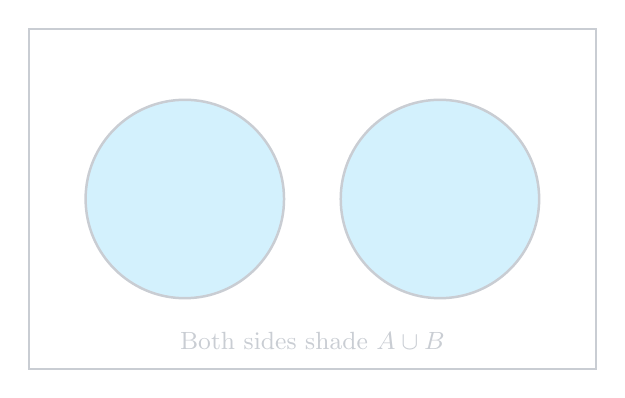
\begin{tikzpicture}[scale=0.9]
  \draw[vennCircle] (-4,-2.4) rectangle (4,2.4);
  \node[vennLabel] at (3.6,2.1) {$C$};

  \def\r{1.4}
  \coordinate (A) at (-1.8,0);
  \coordinate (B) at (1.8,0);

  \fill[vennFill] (A) circle (\r);
  \fill[vennFill] (B) circle (\r);

  \draw[vennCircle] (A) circle (\r);
  \draw[vennCircle] (B) circle (\r);

  \node[vennLabel] at (-1.8,1.7) {$A$};
  \node[vennLabel] at (1.8,1.7) {$B$};

  \node[vennText, text=muted] at (0,-2.0) {Both sides shade $A\cup B$};
\end{tikzpicture}
\end{center}
\end{QAPair}

% ============================================================
% Q6
\begin{QAPair}{Question 6 (Distributive law of $\cap$ over $\cup$)}
\textcolor{gold}{\bfseries Question:} Verify distributive law of intersection over union through Venn diagram for\\
$P=\{a,b,c,d,e\}$,\; $Q=\{c,d,e,f\}$,\; $R=\{g,h,i,j,k\}$.\\
\tcblower
\textcolor{green}{\bfseries Answer:}

\[
Q\cup R=\{c,d,e,f,g,h,i,j,k\}.
\]
\[
P\cap(Q\cup R)=\{a,b,c,d,e\}\cap\{c,d,e,f,g,h,i,j,k\}=\{c,d,e\}.
\]
Also,
\[
P\cap Q=\{c,d,e\},\qquad P\cap R=\varnothing,
\]
so
\[
(P\cap Q)\cup(P\cap R)=\{c,d,e\}.
\]
Hence,
\[
P\cap(Q\cup R)=(P\cap Q)\cup(P\cap R).
\]

\begin{center}
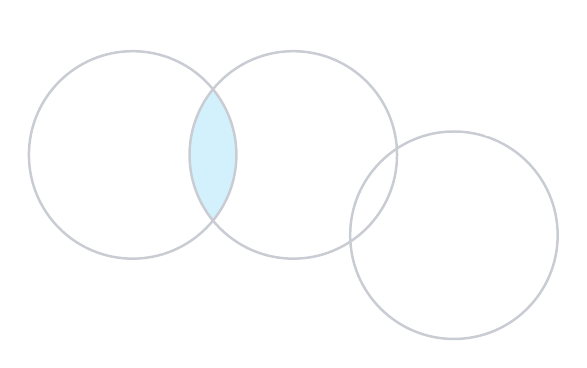
\begin{tikzpicture}[scale=0.85]
  \def\r{1.55}
  \coordinate (P) at (-1.4,0.2);
  \coordinate (Q) at (1.0,0.2);
  \coordinate (R) at (3.4,-1.0);

  \begin{scope}
    \clip (P) circle (\r);
    \fill[vennFill] (Q) circle (\r);
  \end{scope}

  \draw[vennCircle] (P) circle (\r);
  \draw[vennCircle] (Q) circle (\r);
  \draw[vennCircle] (R) circle (\r);

  \node[vennLabel] at (-2.0,1.8) {$P$};
  \node[vennLabel] at (1.6,1.8) {$Q$};
  \node[vennLabel] at (4.0,0.6) {$R$};
\end{tikzpicture}
\end{center}
\end{QAPair}

% ============================================================
% Q7
\begin{QAPair}{Question 7 (Venn diagrams using given numbers)}
\textcolor{gold}{\bfseries Question:} Create a Venn diagram for subsets $A$ and $B$ in the universal set $U$.\\
(i) $n(A)=60$, $n(B)=48$, $n(A\cap B)=20$, $n(U)=90$\\
(ii) $n(A)=34$, $n(B)=52$, $n(A\cup B)=60$, $n(U)=85$\\
\tcblower
\textcolor{green}{\bfseries Answer:}

\textcolor{muted}{\textbf{(i)}}\;
\[
\begin{aligned}
n(A\setminus B)&=60-20=40,\\
n(B\setminus A)&=48-20=28,\\
n(A\cup B)&=60+48-20=88,\\
n(U\setminus(A\cup B))&=90-88=2.
\end{aligned}
\]

\begin{center}
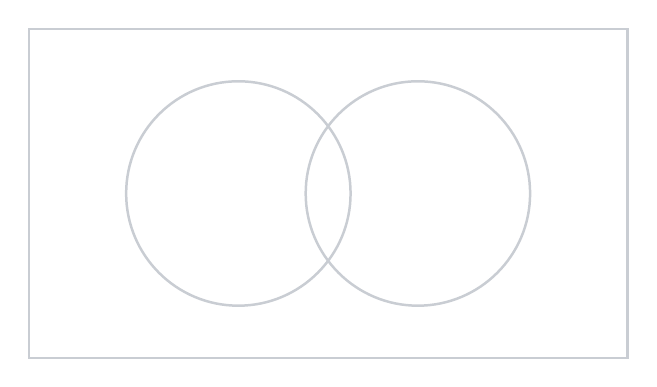
\begin{tikzpicture}[scale=0.95]
  \draw[vennCircle] (-4,-2.2) rectangle (4,2.2);
  \node[vennLabel] at (3.6,1.9) {$U$};

  \def\r{1.5}
  \coordinate (A) at (-1.2,0);
  \coordinate (B) at (1.2,0);

  \draw[vennCircle] (A) circle (\r);
  \draw[vennCircle] (B) circle (\r);

  \node[vennLabel] at (-2.1,1.6) {$A$};
  \node[vennLabel] at (2.1,1.6) {$B$};

  \node[vennText] at (-2.0,0) {\textbf{40}};
  \node[vennText] at (0,0) {\textbf{20}};
  \node[vennText] at (2.0,0) {\textbf{28}};
  \node[vennText] at (0,-1.7) {\textbf{2}};
\end{tikzpicture}
\end{center}

\textcolor{muted}{\textbf{(ii)}}\;
\[
\begin{aligned}
n(A\cap B)&=34+52-60=26,\\
n(A\setminus B)&=34-26=8,\\
n(B\setminus A)&=52-26=26,\\
n(U\setminus(A\cup B))&=85-60=25.
\end{aligned}
\]

\begin{center}
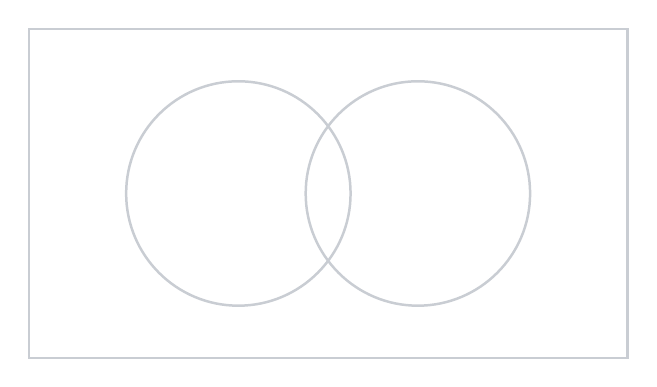
\begin{tikzpicture}[scale=0.95]
  \draw[vennCircle] (-4,-2.2) rectangle (4,2.2);
  \node[vennLabel] at (3.6,1.9) {$U$};

  \def\r{1.5}
  \coordinate (A) at (-1.2,0);
  \coordinate (B) at (1.2,0);

  \draw[vennCircle] (A) circle (\r);
  \draw[vennCircle] (B) circle (\r);

  \node[vennLabel] at (-2.1,1.6) {$A$};
  \node[vennLabel] at (2.1,1.6) {$B$};

  \node[vennText] at (-2.0,0) {\textbf{8}};
  \node[vennText] at (0,0) {\textbf{26}};
  \node[vennText] at (2.0,0) {\textbf{26}};
  \node[vennText] at (0,-1.7) {\textbf{25}};
\end{tikzpicture}
\end{center}
\end{QAPair}

% ============================================================
% Q8
\begin{QAPair}{Question 8 (Qiraat competition sets + Venn diagram)}
\textcolor{gold}{\bfseries Question:} 10 boys participated.\\
$A$ (Naafi): Haani, Zubair, Haider\\
$B$ (Al-Kissai): Abdullah, Umer, Bilal, Ali\\
$C$ (Al-Kufi): Hassan, Jaffer, Usman\\
Find (i)--(iii).\\
\tcblower
\textcolor{green}{\bfseries Answer:}

Let
\[
U=\{\text{Haani, Zubair, Haider, Abdullah, Umer, Bilal, Ali, Hassan, Jaffer, Usman}\}.
\]

\begin{enumerate}[label=\textbf{(\roman*)}]
\item \textbf{Tabular form:}
\[
\begin{aligned}
A&=\{\text{Haani, Zubair, Haider}\},\\
B&=\{\text{Abdullah, Umer, Bilal, Ali}\},\\
C&=\{\text{Hassan, Jaffer, Usman}\}.
\end{aligned}
\]

\item \textbf{Venn diagram:} (here $A,B,C$ are disjoint)
\begin{center}
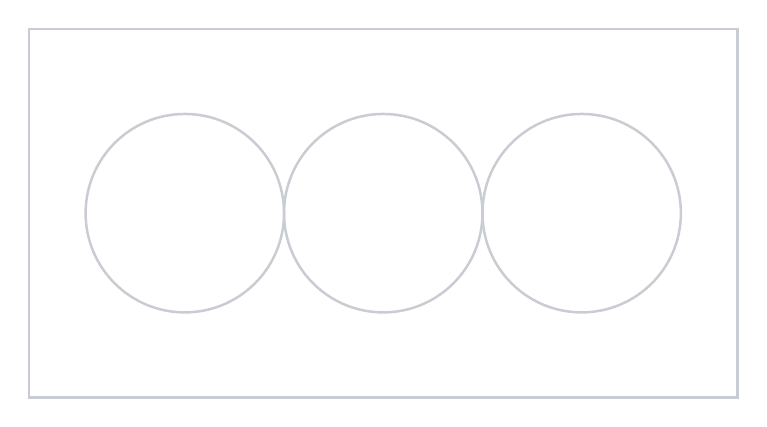
\begin{tikzpicture}[scale=0.9]
  \draw[vennCircle] (-5,-2.6) rectangle (5,2.6);
  \node[vennLabel] at (4.6,2.2) {$U$};

  \def\r{1.4}
  \coordinate (A) at (-2.8,0);
  \coordinate (B) at (0,0);
  \coordinate (C) at (2.8,0);

  \draw[vennCircle] (A) circle (\r);
  \draw[vennCircle] (B) circle (\r);
  \draw[vennCircle] (C) circle (\r);

  \node[vennLabel] at (-2.8,1.6) {$A$};
  \node[vennLabel] at (0,1.6) {$B$};
  \node[vennLabel] at (2.8,1.6) {$C$};

  \node[vennText] at (-2.8,0.35) {\scriptsize Haani};
  \node[vennText] at (-2.8,0.00) {\scriptsize Zubair};
  \node[vennText] at (-2.8,-0.35) {\scriptsize Haider};

  \node[vennText] at (0,0.45) {\scriptsize Abdullah};
  \node[vennText] at (0,0.15) {\scriptsize Umer};
  \node[vennText] at (0,-0.15) {\scriptsize Bilal};
  \node[vennText] at (0,-0.45) {\scriptsize Ali};

  \node[vennText] at (2.8,0.25) {\scriptsize Hassan};
  \node[vennText] at (2.8,-0.05) {\scriptsize Jaffer};
  \node[vennText] at (2.8,-0.35) {\scriptsize Usman};
\end{tikzpicture}
\end{center}

\item \textbf{Find the given expressions} (complements w.r.t. $U$):

Since $B$ and $C$ are disjoint, $B\cap C=\varnothing$ and $(B\cap C)^c=U$.

\[
\begin{aligned}
A\cap(B\cap C)^c &= A\cap U = A,\\
(A\cup B)\cap C^c &= (A\cup B)\cap(U-C) = A\cup B,\\
A-(B\cap C) &= A-\varnothing = A,\\
A-(A\cup B) &= \varnothing.
\end{aligned}
\]
\end{enumerate}
\end{QAPair}

% ============================================================
% Q9
\begin{QAPair}{Question 9 (Three-subject Venn diagram)}
\textcolor{gold}{\bfseries Question:} 100 candidates. Passed in Mathematics (M)=45, Science (S)=40, Health (H)=50.\\
Passed in: $M\cap S=12$, $S\cap H=15$, $H\cap M=20$, and all three $M\cap S\cap H=5$.\\
(i) Draw Venn diagram. (ii) How many passed at least one? (iii) How many did not pass any?\\
\tcblower
\textcolor{green}{\bfseries Answer:}

\textcolor{muted}{\bfseries Step 1: Find pairwise-only regions.}\par
\[
\begin{aligned}
|M\cap S \text{ only}| &= 12-5=7,\\
|S\cap H \text{ only}| &= 15-5=10,\\
|H\cap M \text{ only}| &= 20-5=15.
\end{aligned}
\]

\textcolor{muted}{\bfseries Step 2: Find only-subject regions.}\par
\[
\begin{aligned}
|M\text{ only}| &= 45-(7+15+5)=18,\\
|S\text{ only}| &= 40-(7+10+5)=18,\\
|H\text{ only}| &= 50-(15+10+5)=20.
\end{aligned}
\]

\textcolor{muted}{\bfseries Step 3: Passed at least one.}\par
\[
|M\cup S\cup H| = 18+18+20+7+10+15+5=93.
\]

\textcolor{muted}{\bfseries Step 4: Passed none.}\par
\[
|U-(M\cup S\cup H)| = 100-93=7.
\]

\begin{center}
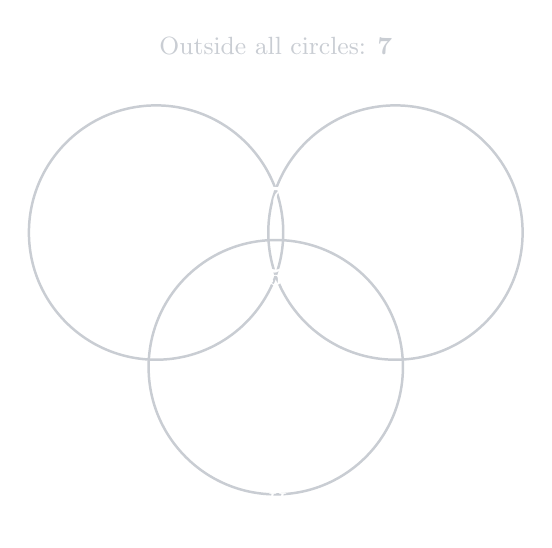
\begin{tikzpicture}[scale=0.95]
  \def\r{1.7}
  \coordinate (M) at (-1.6,0.4);
  \coordinate (S) at (1.6,0.4);
  \coordinate (H) at (0,-1.4);

  \draw[vennCircle] (M) circle (\r);
  \draw[vennCircle] (S) circle (\r);
  \draw[vennCircle] (H) circle (\r);

  \node[vennLabel] at (-2.6,2.2) {$M$};
  \node[vennLabel] at (2.6,2.2) {$S$};
  \node[vennLabel] at (0,-3.2) {$H$};

  \node[vennText] at (-2.9,0.5) {\textbf{18}};
  \node[vennText] at (2.9,0.5) {\textbf{18}};
  \node[vennText] at (0,-2.7) {\textbf{20}};

  \node[vennText] at (0,0.9) {\textbf{7}};
  \node[vennText] at (1.2,-0.9) {\textbf{10}};
  \node[vennText] at (-1.2,-0.9) {\textbf{15}};

  \node[vennText] at (0,-0.2) {\textbf{5}};

  \node[vennText, text=muted] at (0,2.9) {Outside all circles: \textbf{7}};
\end{tikzpicture}
\end{center}
\end{QAPair}

\end{document}
